%%%%%%%%%%%%%%%%%%%%%%%%%%%%%%%%%%%%%%%%%
% Beamer Presentation
% LaTeX Template
% Version 1.0 (10/11/12)
%
% This template has been downloaded from:
% http://www.LaTeXTemplates.com
%
% License:
% CC BY-NC-SA 3.0 (http://creativecommons.org/licenses/by-nc-sa/3.0/)
%
%%%%%%%%%%%%%%%%%%%%%%%%%%%%%%%%%%%%%%%%%

%----------------------------------------------------------------------------------------
%	PACKAGES AND THEMES
%----------------------------------------------------------------------------------------

\documentclass{beamer}

\mode<presentation> {

% The Beamer class comes with a number of default slide themes
% which change the colors and layouts of slides. Below this is a list
% of all the themes, uncomment each in turn to see what they look like.

%\usetheme{default}
%\usetheme{AnnArbor}
%\usetheme{Antibes}
%\usetheme{Bergen}
%\usetheme{Berkeley}
%\usetheme{Berlin}
%\usetheme{Boadilla}
%\usetheme{CambridgeUS}
%\usetheme{Copenhagen}
%\usetheme{Darmstadt}
%\usetheme{Dresden}
%\usetheme{Frankfurt}
%\usetheme{Goettingen}
%\usetheme{Hannover}
%\usetheme{Ilmenau}
%\usetheme{JuanLesPins}
%\usetheme{Luebeck}
\usetheme{Madrid}
%\usetheme{Malmoe}
%\usetheme{Marburg}
%\usetheme{Montpellier}
%\usetheme{PaloAlto}
%\usetheme{Pittsburgh}
%\usetheme{Rochester}
%\usetheme{Singapore}
%\usetheme{Szeged}
%\usetheme{Warsaw}

% As well as themes, the Beamer class has a number of color themes
% for any slide theme. Uncomment each of these in turn to see how it
% changes the colors of your current slide theme.

%\usecolortheme{albatross}
%\usecolortheme{beaver}
%\usecolortheme{beetle}
%\usecolortheme{crane}
%\usecolortheme{dolphin}
%\usecolortheme{dove}
%\usecolortheme{fly}
%\usecolortheme{lily}
%\usecolortheme{orchid}
%\usecolortheme{rose}
%\usecolortheme{seagull}
%\usecolortheme{seahorse}
%\usecolortheme{whale}
%\usecolortheme{wolverine}

%\setbeamertemplate{footline} % To remove the footer line in all slides uncomment this line
%\setbeamertemplate{footline}[page number] % To replace the footer line in all slides with a simple slide count uncomment this line

%\setbeamertemplate{navigation symbols}{} % To remove the navigation symbols from the bottom of all slides uncomment this line
}

\usepackage{graphicx} % Allows including images
\usepackage{booktabs} % Allows the use of \toprule, \midrule and \bottomrule in tables

%----------------------------------------------------------------------------------------
%	TITLE PAGE
%----------------------------------------------------------------------------------------

\title[FiQuant Market Simulator]{Market Microstructure Simulator: Strategy Definition Language} % The short title appears at the bottom of every slide, the full title is only on the title page

\author{Anton Kolotaev} % Your name
\institute[ECP] % Your institution as it will appear on the bottom of every slide, may be shorthand to save space
{
Chair of Quantitative Finance, \'{E}cole Centrale Paris \\ % Your institution for the title page
\medskip
\textit{anton.kolotaev@gmail.com} % Your email address
}
\date{\today} % Date, can be changed to a custom date

\begin{document}

\begin{frame}
\titlepage % Print the title page as the first slide
\end{frame}

\begin{frame}
\frametitle{Overview} % Table of contents slide, comment this block out to remove it
\tableofcontents % Throughout your presentation, if you choose to use \section{} and \subsection{} commands, these will automatically be printed on this slide as an overview of your presentation
\end{frame}

%----------------------------------------------------------------------------------------
%	PRESENTATION SLIDES
%----------------------------------------------------------------------------------------

%------------------------------------------------
\section{Introduction}

%------------------------------------------------
\begin{frame}
\frametitle{Evolution of the simulator I}
\begin{enumerate}
  \item Initial C++ version was developed in 2009-2011 by Riadh Zaatour. In this version a user implements strategy logic in C++. Though this version was quite easy to learn and understand, it had problems with flexibility and scalability.
  \item In order to improve its extensibility and performance the simulator was rewritten using C++ template metaprogramming techniques by Anton Kolotaev in 2012. Python bindings to it were implemented using Boost.Python. Unfortunately the price for providing high extensibility with no overhead was quite high: in order to use it a proficiency in C++ template metaprogramming was required.
\end{enumerate}
\end{frame}
%------------------------------------------------
\begin{frame}
\frametitle{Evolution of the simulator II}
\begin{enumerate}
  \item In order to make the simulator easy to to start work with, a Python version with a Web interface was developed in 2013. Karol Podkanski implemented number of trading strategies and indicators during his internship at summer 2013. Though this version gave a lot of insights on how a good modular design for market simulation software should be implemented, it showed that a lot of syntax noise appears in strategy description and the development becomes very error-prone because of the dynamic typing nature of Python.
  \item In October 2013 a decision to introduce a strategy definition language and a compiler for it was taken.
\end{enumerate}
\end{frame}
%------------------------------------------------
\begin{frame}
\frametitle{Design goals}
\begin{enumerate}
  \item \textbf{\textit{Flexibility}}. A simulation library must have a very modular design in order to provide a high level of flexibility to the user. This requirement comes from the original purpose of a simulation as a test bed for experiments with different models and parameters.
  \item \textbf{\textit{Used-friendliness}}. Since a typical simulation model is composed of many hundreds and thousands blocks, it is very important to provide a simple way for user to tell how a behaviour wanted differs from the default one. Simulator API should be friendly to modern IDEs
  \item \textbf{\textit{Performance}}. A used should be allowed to choose between small start-up time and high simulation speed.
\end{enumerate}
\end{frame}
%------------------------------------------------
\begin{frame}
\frametitle{Modular Design}
Representing a simulation model as a \textbf{network} of modules communicating by \textbf{messages} is a widely accepted practice for DES systems (e.g. Omnet++ or ns-2 for telecommunication network simulations).

Module may have \textbf{parameters} that are used to adjust their behaviour. Modules may be organized into \textbf{hierarchy} in order to facilitate construction of large-scale simulation and it is useful to distinguish two sorts of modules:
\begin{enumerate}
\item \textbf{\textit{Simple modules}} provide functionality which is considered elementary (and there is no reason to reuse part of it to implement other modules).

\item \textbf{\textit{Compound modules}} combine together other modules in some way and define their parameters based on its own parameters. Compound module behaviour is just a composition of its constituting modules behaviours.
\end{enumerate}
\end{frame}
%------------------------------------------------

\begin{frame}
\frametitle{Modular design sample}
\begin{figure}[htbp]
\centering
\includegraphics[width=1\linewidth]{graph.png}
\end{figure}
\end{frame}
%------------------------------------------------
\begin{frame}
\frametitle{Motivation for an external DSL}
\begin{enumerate}
  \item \textbf{\textit{Syntax}}. We may design an external DSL so its syntax describes very well domain specific abstraction.
  \item \textbf{\textit{Error checking}}. A DSL compiler can detect incorrect parameter values as soon as possible thus shortening simulation development cycle and facilitating refactorings.
  \item \textbf{\textit{Multiple target languages}}. A DSL can be compiled into different languages: e.g. into Python to provide fast start-up and into C++ to have highly optimized simulations. A new target language introduced, only simple modules need to be re-written into it; compound modules will be ported automatically.
  \item \textbf{\textit{IDE support}}. Modern IDEs like Eclipse, Intellij IDEA allow writing plug-ins that would provide smart syntax highlighting, auto-completion and check errors on-the-fly for user-defined DSLs.
  \item \textbf{\textit{High-level optimizations}}. 
\end{enumerate}
\end{frame}
%------------------------------------------------
\begin{frame}
\frametitle{Scala as a language to implement the DSL compiler}
\begin{enumerate}
  \item As a ML-family member, very suitable for sophisticated symbol processing tasks like compilation: an internal DSL to parse texts, algebraic data types, pattern matching, a powerful collections library, mixin inheritance via traits.
  \item Good balance between functional and imperative programming features -- easier to find software engineers
  \item The most mainstream of a functional programming languages that results in wide community, excellent library and tool support, mature IDEs.
  \item Very portable since runs on JVM.
  \item Statically typed
  \item Right choice to develop a Web server.
\end{enumerate}
\end{frame}
%------------------------------------------------
\begin{frame}
\frametitle{Functions}
Conceptually, a "function" declaration defines a term with a constructor provided (like case classes in Scala). 

Types for input arguments are inferred automatically from their initializers and for the "return" value - from the function body.

Functions represent compound modules of a simulation model.

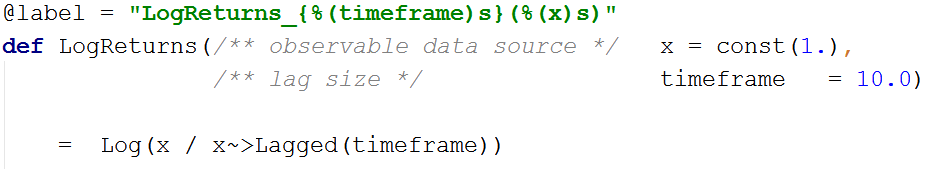
\includegraphics[width=1\linewidth]{logreturns.png}

All methods are considered as extension methods of their first argument.
\end{frame}
%------------------------------------------------
\begin{frame}
\frametitle{Intrinsic Functions}
Intrinsic functions import simple modules from a target language into the DSL. 
"Return" types for intrinsic functions must be specified explicitly.
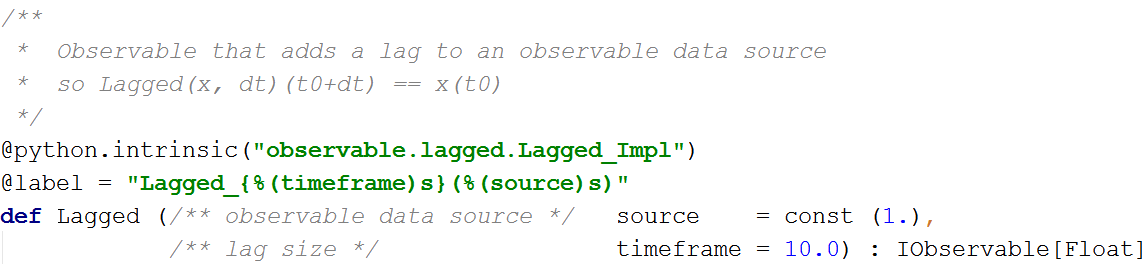
\includegraphics[width=1\linewidth]{lagged.png}
\end{frame}
%------------------------------------------------
\begin{frame}
\frametitle{Type System I}
Types correspond to interfaces without methods from mainstream languages. They are used for error checking and for function overloading.
\begin{enumerate}
  \item Simple types may derive from other types or be aliases
  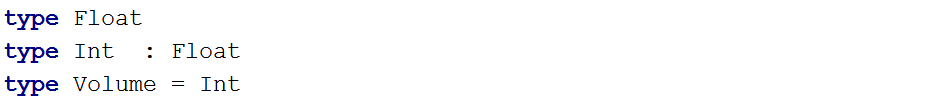
\includegraphics[width=1\linewidth]{intfloat.png}
  \item Tuple and function types
  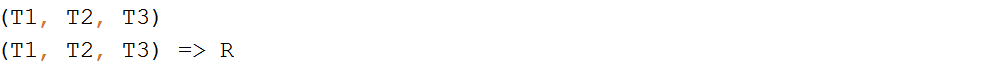
\includegraphics[width=1\linewidth]{tuplefunction.png}
  \item Top (\texttt{Any}) and bottom (\texttt{Nothing}) types.
  \item Lists (\texttt{List[T]})
\end{enumerate}
\end{frame}
%------------------------------------------------
\begin{frame}
\frametitle{Type System II}
Types may be generic. 

Functions are contravariant in the input type and covariant in the output type: \texttt{CanCast(D,B)} $\wedge$ \texttt{CanCast(R,T)} $\Rightarrow$ \texttt{CanCast(B=>R,D=>T)}.

All other types are covariant.

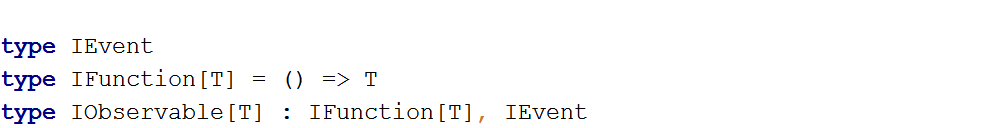
\includegraphics[width=1\linewidth]{iobservable.png}

\end{frame}
%------------------------------------------------

\begin{frame}
\frametitle{Classes I}
Classes are syntax sugar for a type declaration, constructor function and member accessors

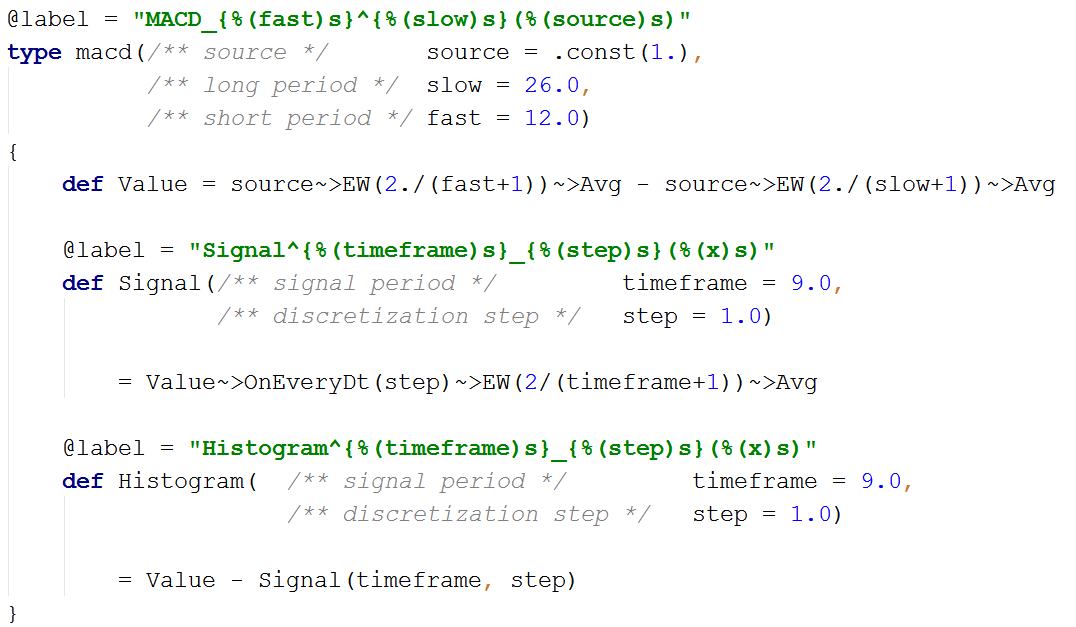
\includegraphics[width=1\linewidth]{macd.png}

\end{frame}
%------------------------------------------------
\begin{frame}
\frametitle{Classes II}
Previous definition is de-sugared at typing stage into

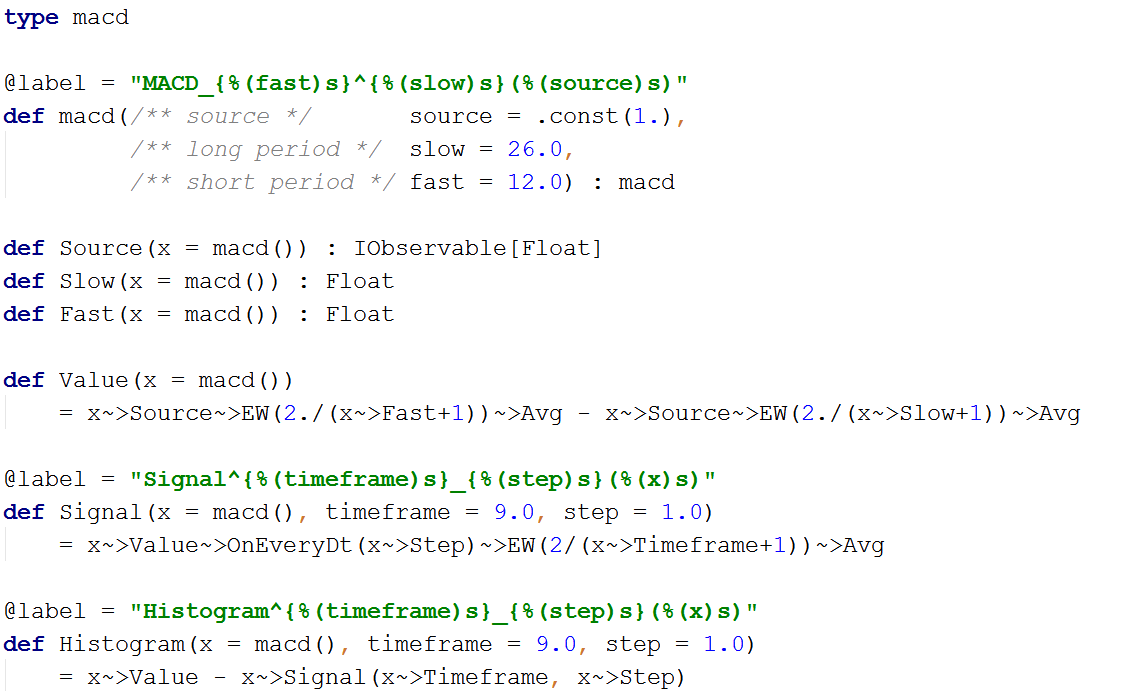
\includegraphics[width=1\linewidth]{macd_desugared.png}
\end{frame}
%------------------------------------------------
\begin{frame}
\frametitle{Class Inheritance}
Classes derive fields and methods from base classes.

Methods are treated as "virtual" to stimulate code re-use

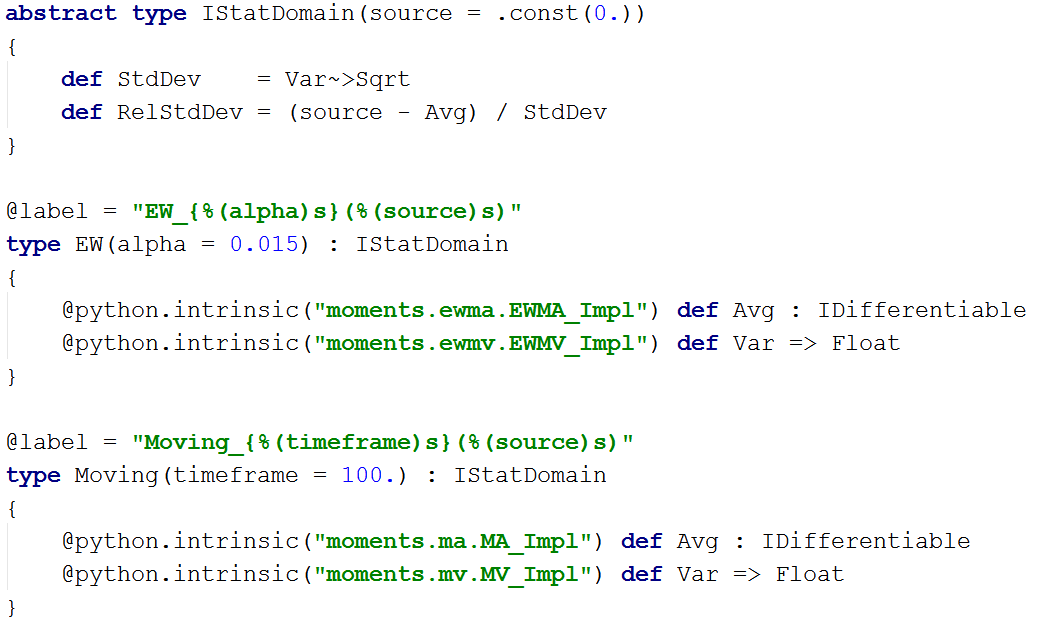
\includegraphics[width=1\linewidth]{moments.png}
\end{frame}
%------------------------------------------------
\begin{frame}
\frametitle{Packages and Attributes}
Package are used to group functions and types. They can be nested. Attributes are inherited from enclosing package. Anonymous packages are used to assign same attributes to a group of functions without introducing a new name scope.

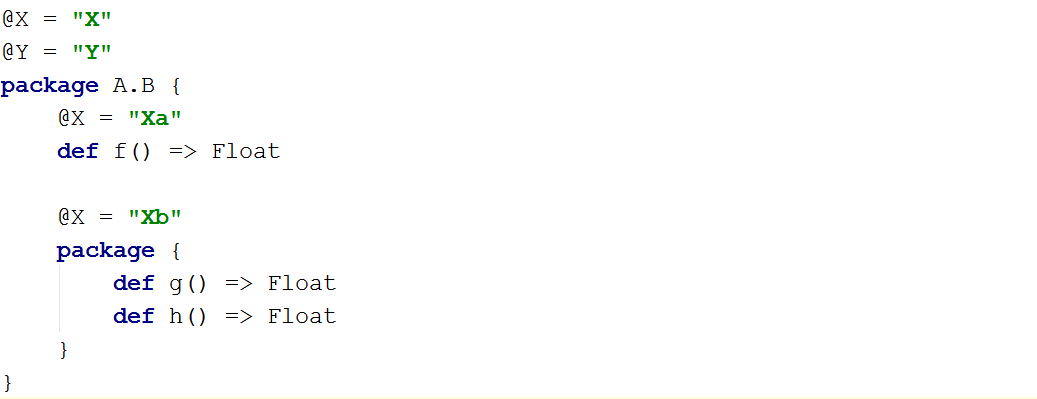
\includegraphics[width=1\linewidth]{packages.png}

In this sample \texttt{.A.B.f} will have attributes \texttt{X == "Xa", Y == "Y"} and \texttt{.A.B.g} and \texttt{.A.B.h} will have attributes \texttt{X == "Xb", Y == "Y"}

\end{frame}
%------------------------------------------------
\begin{frame}
\frametitle{Example: Relative Strength Index}
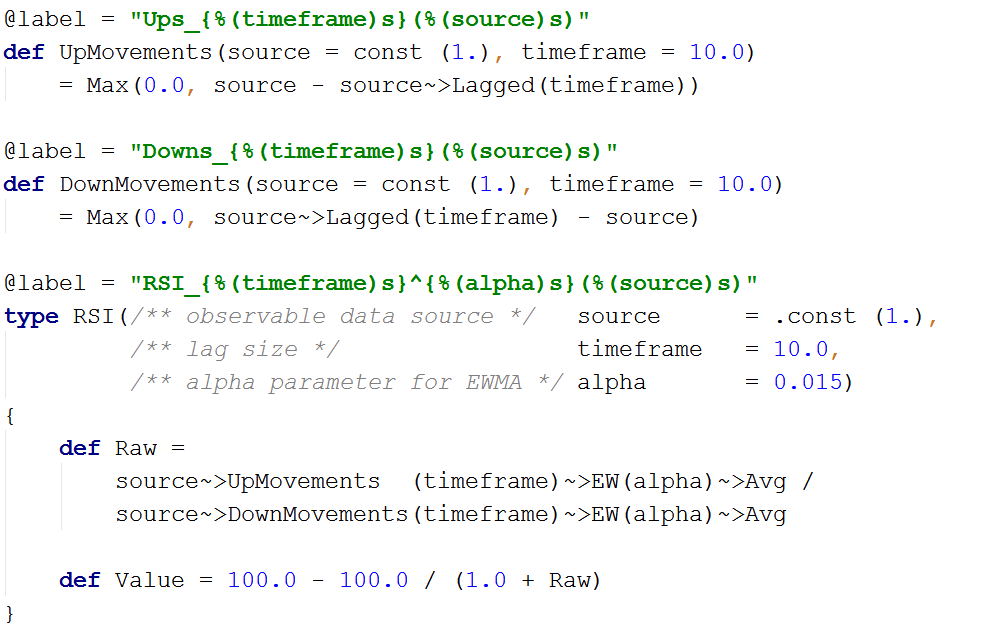
\includegraphics[width=1\linewidth]{rsi.png}
\end{frame}
%------------------------------------------------
\begin{frame}
\frametitle{Example: Relative Strength Index Strategy}
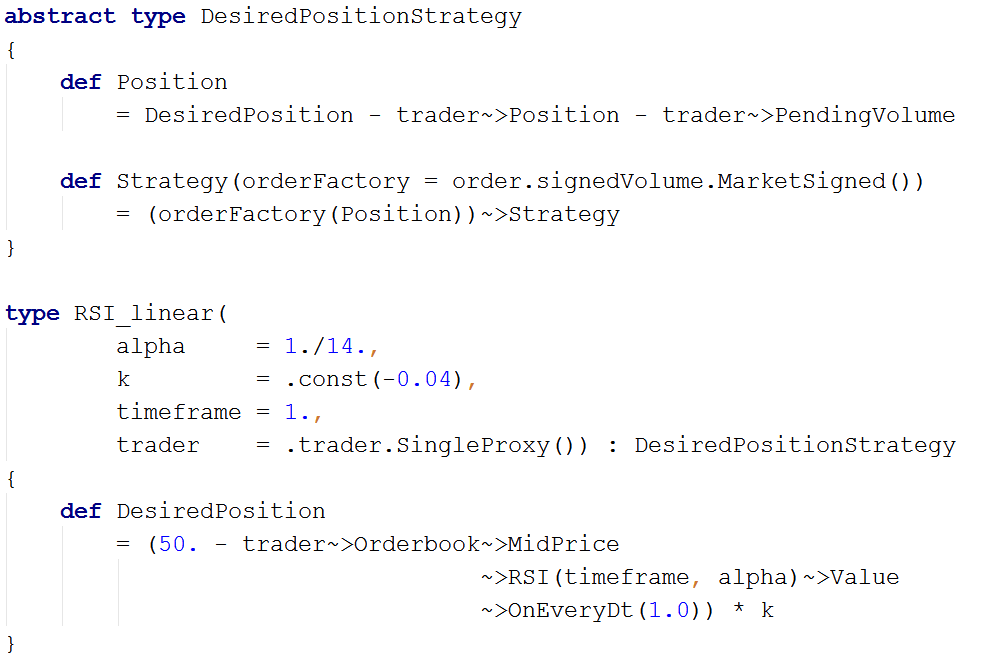
\includegraphics[width=1\linewidth]{rsi_strategy.png}
\end{frame}
%------------------------------------------------

\begin{frame}
\frametitle{Installation}
\begin{itemize}
\item OS supported: Linux, Mac OS X, Windows
\item Browsers supported: Chrome, Firefox, Safari, Opera
\item Python 2.7
\item Python packages can be installed using \texttt{pip} or \texttt{easyinstall}:
\begin{itemize}
\item \textcolor[rgb]{0.00,0.50,0.75}{\href{http://home.gna.org/veusz/}{Veusz}} (for graph plotting)
\item \textcolor[rgb]{0.00,0.50,0.75}{\href{http://flask.pocoo.org}{Flask}} (to run a Web-server)
\item \textcolor[rgb]{0.00,0.50,0.75}{\href{https://pypi.python.org/pypi/blist/}{Blist}} (sorted collections used by ArbitrageTrader)
\end{itemize}
\item Source code downloadable from \textcolor[rgb]{0.00,0.50,0.75}{\href{http://sourceforge.net/p/marketsimulator/svn/HEAD/tree/DevAnton/v3/}{SourceForge}}
\end{itemize}

\end{frame}

\section{Simulator components}

\begin{frame}
\frametitle{Simulator components}
\begin{figure}[htbp]
\centering
\includegraphics[width=1\linewidth]{objects.png}
\end{figure}
\end{frame}

\subsection{Scheduler}
\begin{frame}
\frametitle{Scheduler}
\begin{itemize}
  \item Main class for every discrete event simulation system.
  \item Maintains a set of actions to fulfill in future and launches them according their action times: from older ones to newer.
\end{itemize}
Interface:
\begin{itemize}
  \item Event scheduling:
  \begin{itemize}
    \item \texttt{schedule(actionTime, handler)}
    \item \texttt{scheduleAfter(dt, handler)}
  \end{itemize}
  \item Simulation control:
  \begin{itemize}
    \item \texttt{workTill(limitTime)}
    \item \texttt{advance(dt)}
    \item \texttt{reset()}
  \end{itemize}
\end{itemize}
\end{frame}

%------------------------------------------------
\subsection{Order books} % A subsection can be created just before a set of slides with a common theme to further break down your presentation into chunks
\begin{frame}
\frametitle{Order book}
\begin{itemize}
  \item Represents a single asset traded in some market (Same asset traded in different markets would be represented by different order books)
  \item Matches incoming orders
  \item Stores unfulfilled limit orders in two order queues (\texttt{Asks} for sell orders and \texttt{Bids} for buy orders)
  \item Corrects limit order price with respect to tick size
  \item Imposes order processing fee
  \item Supports queries about order book structure
  \item Notifies listeners about trades and price changes
\end{itemize}
\end{frame}

%------------------------------------------------
\begin{frame}
\frametitle{Order book for a remote trader}
\begin{itemize}
  \item Models a trader connected to a market by a communication channel with non-negligible latency
  \item Introduces delay in information propagation from a trader to an order book and vice versa (so a trader has outdated information about market and orders are sent to the market with a certain delay)
  \item Assures correct order of messages: older messages always come earlier than newer ones
\end{itemize}
\end{frame}

%------------------------------------------------
\subsection{Orders}
\begin{frame}
\frametitle{Basic orders}
Orders supported internally by an order book:
\begin{itemize}
  \item \texttt{Market(side, volume)}
  \item \texttt{Limit(side, price, volume)}
  \item \texttt{Cancel(limitOrder)}
\end{itemize}
Limit and market orders notifies their listeners about all trades they take part in.
Factory functions are usually used in order to create orders.
\end{frame}

%------------------------------------------------
\begin{frame}
\frametitle{Meta orders}
Follow order interface from trader's perspective (so they can be used instead of basic orders) but behave like a sequence of base orders from an order book point of view.
\begin{itemize}
  \item \texttt{Iceberg(volumeLimit, orderToSplit)} splits \texttt{orderToSplit} to pieces with volume less than \texttt{volumeLimit} and sends them one by one to an order book ensuring that only one order at time is processed there
  \item \texttt{AlwaysBest(volume, limitOrderFactory)} creates a limit-like order with given volume and the most attractive price, sends it to an order book and if the order book best price changes, cancels it and resends with a better price
  \item \texttt{WithExpiry(lifetime, limitOrderFactory)} sends a limit-like order and after \texttt{lifetime} cancels it
  \item \texttt{LimitMarket(limitOrderFactory)} is like \texttt{WithExpiry} but with \texttt{lifetime} equal to 0
\end{itemize}
\end{frame}

%------------------------------------------------
\subsection{Traders}
\begin{frame}
\frametitle{Traders}
Single asset traders
\begin{itemize}
  \item send orders to order books
  \item bookkeep their position and balance
  \item run a number of trading strategies
  \item notify listeners about trades done and orders sent
\end{itemize}
Single asset traders operate on a single or multiple markets.
Multiple asset traders are about to be added.
\end{frame}

%------------------------------------------------
\subsection{Strategies}
\begin{frame}
\frametitle{Generic strategy}
Generic strategy that wakes up on events given by \texttt{eventGen},
chooses side of order to create using \texttt{sideFunc} and its volume by \texttt{volumeFunc},
creates an order via \texttt{orderFactory} and sends the order to the market using its trader
\begin{figure}[htbp]
\centering
\includegraphics[width=9cm, height=5cm]{python-generic.png}
\end{figure}
\end{frame}

%------------------------------------------------

\begin{frame}
\frametitle{Signal strategy}
Signal strategy listens to some discrete signal and when the signal becomes more than some threshold it starts to buy. When the signal gets lower than -threshold the strategy starts to sell.
\begin{figure}[htbp]
\centering
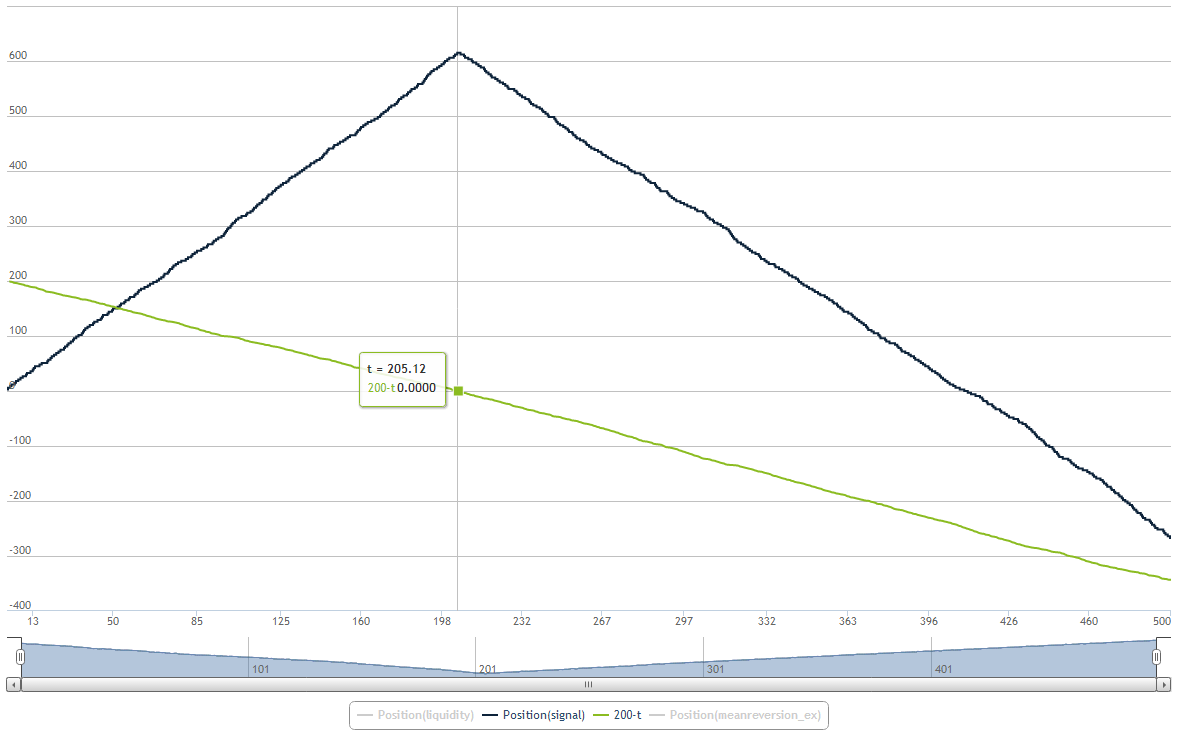
\includegraphics[width=1\linewidth]{signal.png}
\end{figure}
\end{frame}

%------------------------------------------------

\begin{frame}
\frametitle{Trend follower strategy}
Trend follower is an instance of a signal strategy with signal equal to the first derivative of a moving average of the asset's price (i.e trend).
\begin{figure}[htbp]
\centering
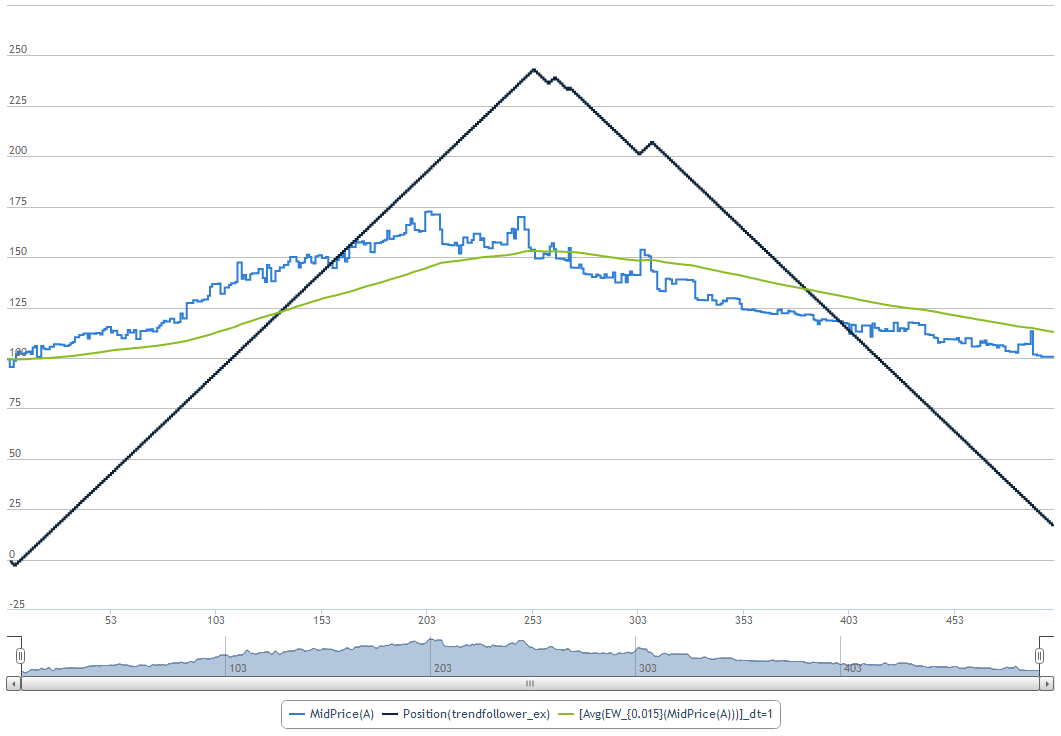
\includegraphics[width=1\linewidth]{trendfollower.png}
\end{figure}
\end{frame}

%------------------------------------------------

\begin{frame}
\frametitle{Two averages strategy}
Two averages is an instance of a signal strategy with signal equal to the difference between two moving averages of the asset's price (i.e trend).
\begin{figure}[htbp]
\centering
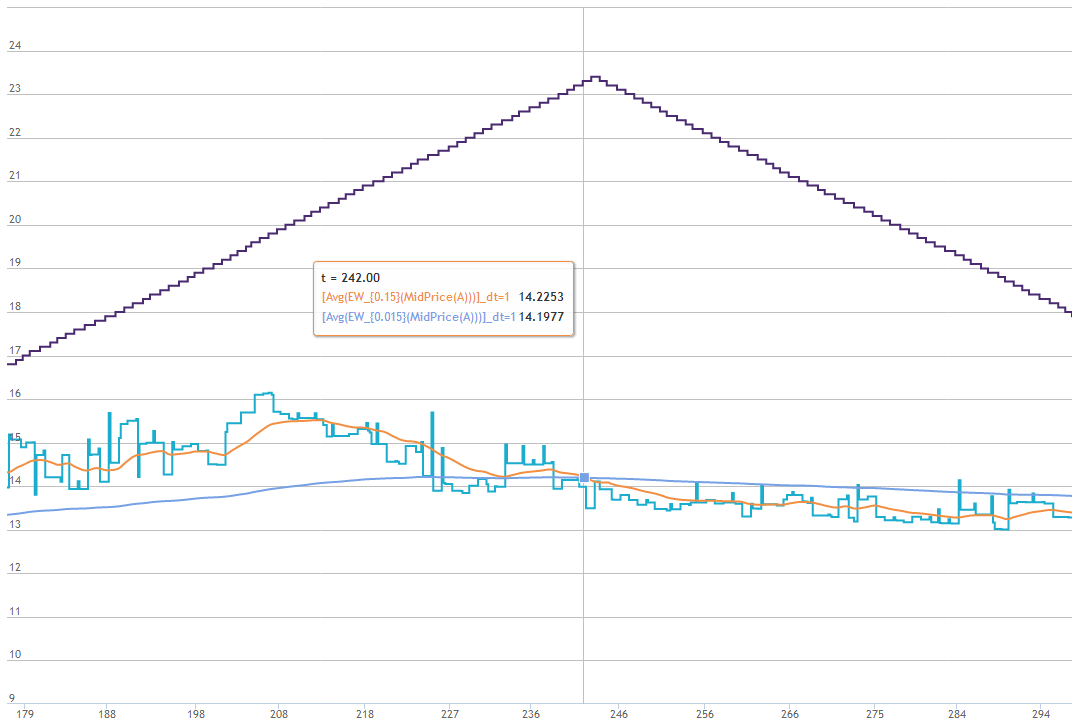
\includegraphics[width=1\linewidth]{twoaverages.png}
\end{figure}
\end{frame}
%------------------------------------------------

\begin{frame}
\frametitle{Fundamental value strategy}
Fundamental value strategy is an instance of a signal strategy with signal equal to the difference between the asset's price and some fundamental value.
\begin{figure}[htbp]
\centering
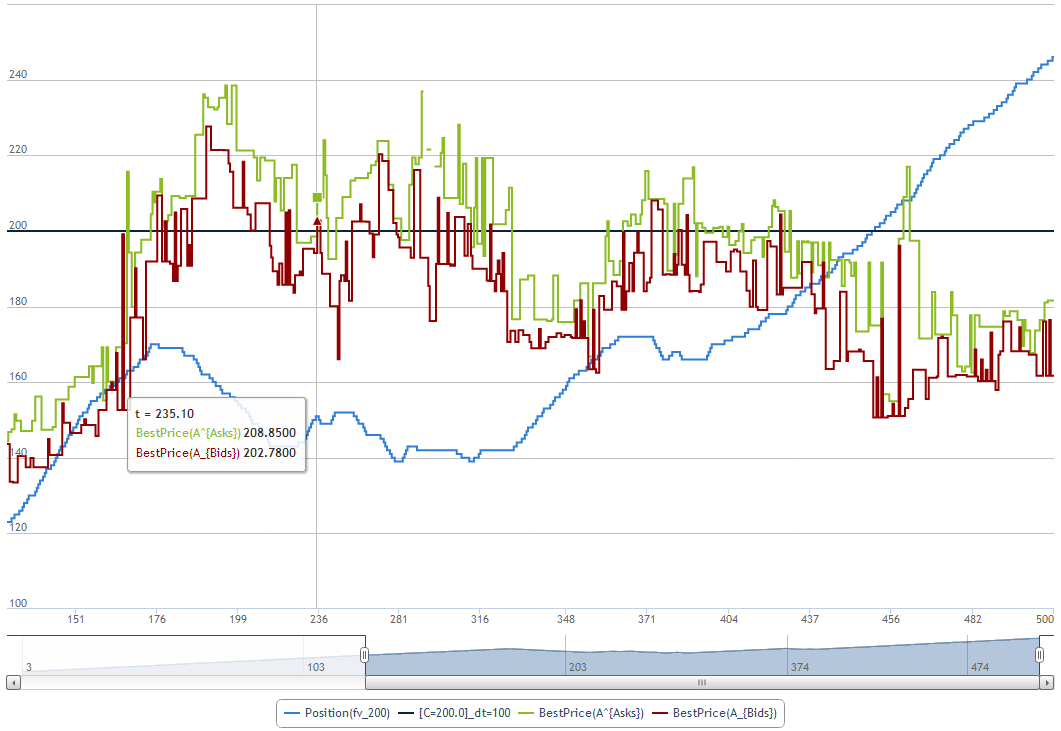
\includegraphics[width=1\linewidth]{fundamentalvalue.png}
\end{figure}
\end{frame}
%------------------------------------------------

\begin{frame}
\frametitle{Mean reversion strategy}
Mean reversion strategy is an instance of a fundamental value strategy with fundamental value equal to some moving average of the asset's price.
\begin{figure}[htbp]
\centering
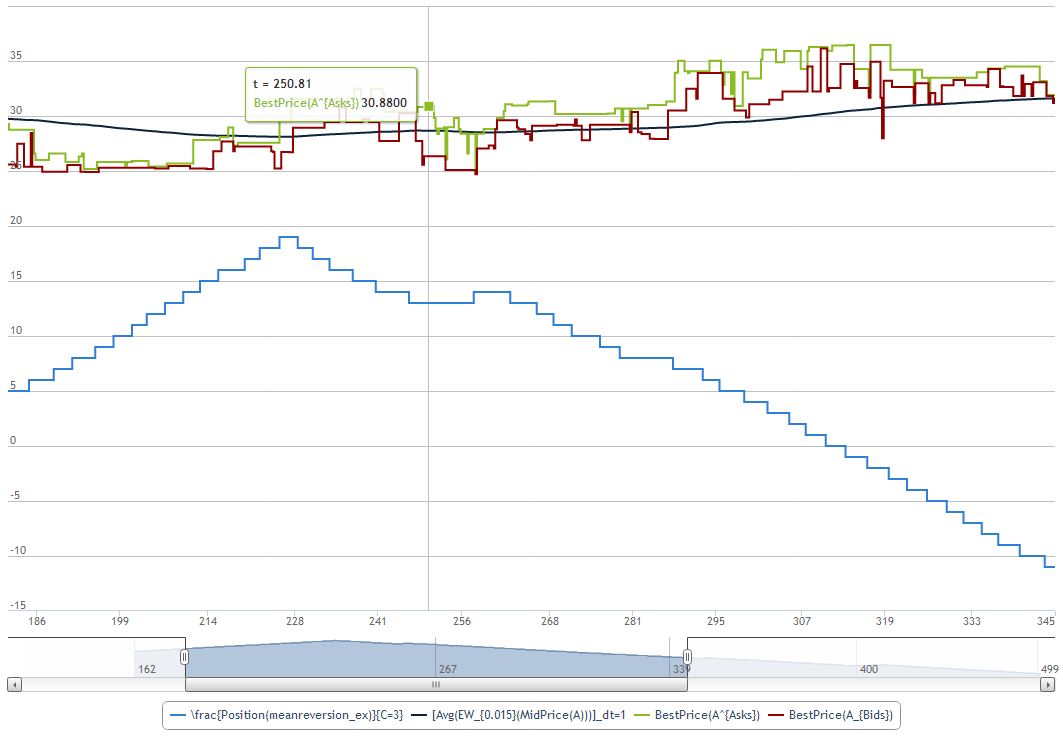
\includegraphics[width=1\linewidth]{meanreversion.png}
\end{figure}
\end{frame}
%------------------------------------------------

\begin{frame}
\frametitle{Dependency strategy}
Dependency strategy is an instance of a fundamental value strategy with fundamental value equal to another asset's price multiplied by given factor.
\begin{figure}[htbp]
\centering
\includegraphics[width=1\linewidth]{dependency.png}
\end{figure}
\end{frame}
%------------------------------------------------

\begin{frame}
\frametitle{Liquidity provider}
Liquidity provider sends limit-like orders with a price equal to the current asset's price multiplied by some randomly chosen factor
\begin{figure}[htbp]
\centering
\includegraphics[width=1\linewidth]{liquidityprovider.png}
\end{figure}
\end{frame}
%------------------------------------------------

\begin{frame}
\frametitle{Trade-if-profitable strategy}
Suspends or resumes an underlying strategy basing on its performance backtesting. By default, first derivative of a moving average of 'cleared' trader's balance (trader's balance if its position was cleared) is used to evaluate the efficiency.
\begin{figure}[htbp]
\centering
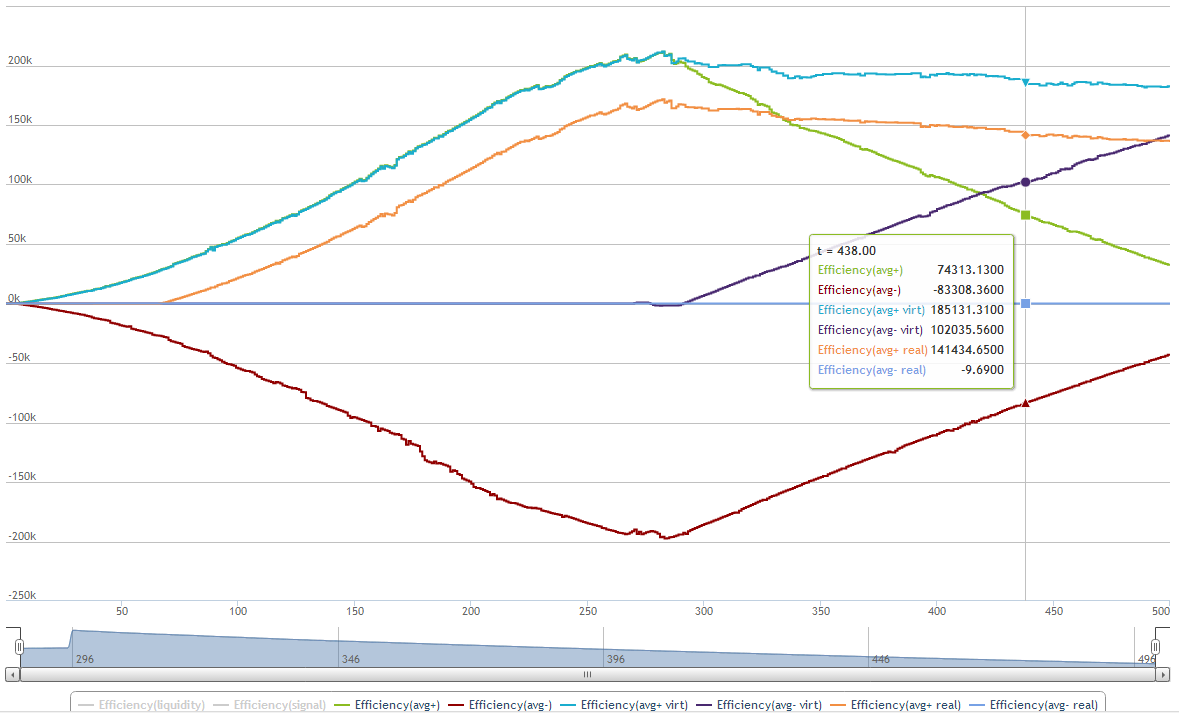
\includegraphics[width=1\linewidth]{tradeifprofitable.png}
\end{figure}
\end{frame}
%------------------------------------------------

\begin{frame}
\frametitle{Choose-the-best strategy}
Backtests aggregated strategies and allows to run only to that one who has the best performance. By default, first derivative of a moving average of 'cleared' trader's balance is used to evaluate the efficiency.
\begin{figure}[htbp]
\centering
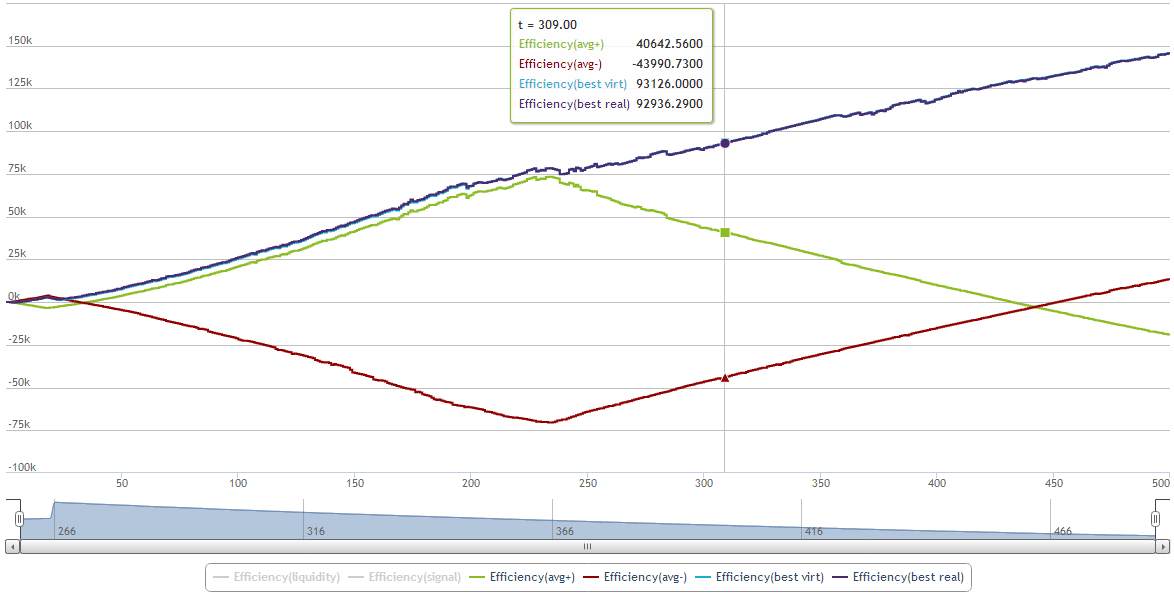
\includegraphics[width=1\linewidth]{choosethebest.png}
\end{figure}
\end{frame}
%------------------------------------------------
\subsection{Observables}
\begin{frame}
\frametitle{Observable}
Traders and order books provide basic accessors to their current state but don't collect any statistics. In order to do it in an interoperable way a notion of observable value was introduced: it allows to read its current value and notifies listeners about its change.
\begin{itemize}
    \item Primitive observables on
    \begin{itemize}
      \item traders: position, balance, market value of the portfolio, 'cleared' balance etc.
      \item order books: ask/mid/bid price, last trade price, price at volume, volume of orders with price better than given one etc.
    \end{itemize}
    \item \texttt{OnEveryDt(dt, dataSource)} evaluates \texttt{dataSource} every \texttt{dt} moments of time. Often used with \texttt{Fold(observable, accumulator)} where \texttt{accumulator} may be a moving average or another statistics collector.
\end{itemize}
History of an observable can be stored in a \texttt{TimeSerie} and rendered later on a graph.
\end{frame}
%------------------------------------------------

\section{Using Veusz}
\begin{frame}
\frametitle{Using Veusz}
When developing a new strategy it is reasonable to test it using scripts and visualize results by Veusz
\begin{figure}[htbp]
\centering
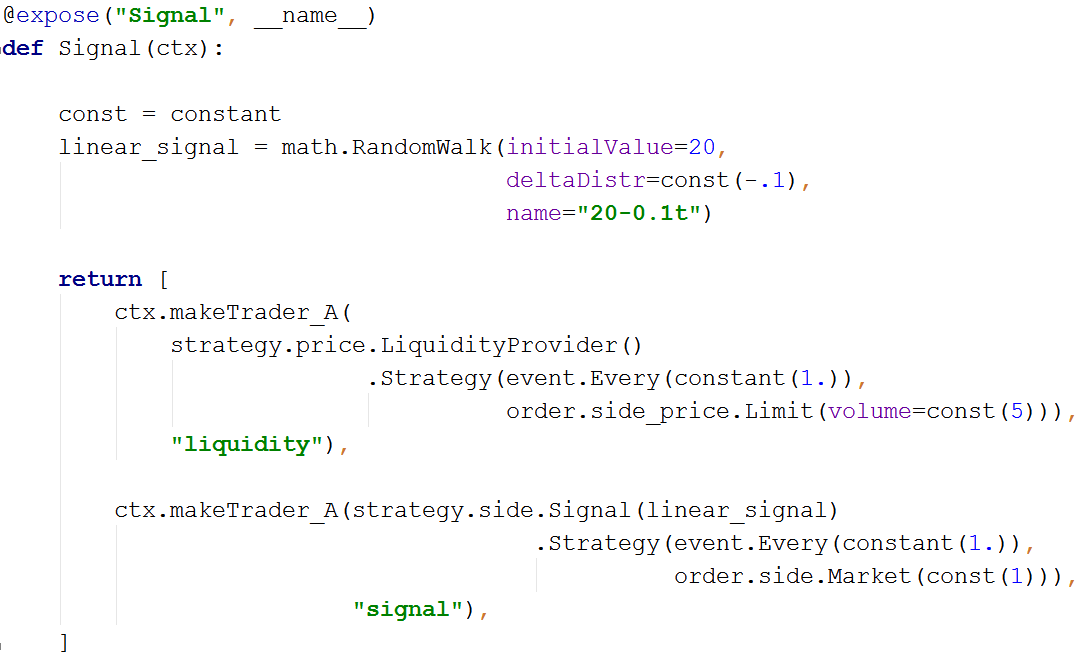
\includegraphics[width=1\linewidth]{using_veusz_code.png}
\end{figure}
\end{frame}

%------------------------------------------------
\begin{frame}
\frametitle{Rendering graphs by Veusz}
\begin{figure}[htbp]
\centering
\includegraphics[width=1\linewidth]{veusz_graph.png}
\end{figure}
\end{frame}

%------------------------------------------------

\section{Web interface}
\begin{frame}
\frametitle{Web interface}
Web interface allows to compose a market to simulate from existing objects and set up their parameters
\begin{figure}[htbp]
\centering
\includegraphics[width=1\linewidth]{js-help.png}
\end{figure}
\end{frame}

\begin{frame}
\frametitle{Time series}
Timeseries field of a trader or an order book instructs what data should be collected and rendered on graphs
\begin{figure}[htbp]
\centering
\includegraphics[width=1\linewidth]{js-timeserie.png}
\end{figure}
\end{frame}

\begin{frame}
\frametitle{Rendering results}
\begin{figure}[htbp]
\centering
\includegraphics[width=1\linewidth]{js-graph.png}
\end{figure}
\end{frame}

\begin{frame}
\frametitle{Node aliases}
\begin{figure}[htbp]
Object tree nodes can be assigned aliases that can be used later to refer to the sub-tree (explicit by-value or by-reference cloning semantics is to be implemented)
\centering
\includegraphics[width=1\linewidth]{js-alias.png}
\end{figure}
\end{frame}

\begin{frame}
\frametitle{Workspaces}
\begin{figure}[htbp]
Every user (identified by browser cookies) may switch between multiple workspaces. Workspaces can be forked, removed or created from a set of predefined ones.
\centering
\includegraphics[width=1\linewidth]{js-fork.png}
\end{figure}
\end{frame}

\section{Exposing Python classes to Web-interface}
\begin{frame}
\frametitle{Exposing Python classes to Web-interface}
\begin{itemize}
  \item displayable label for the class ('Random Walk')
  \item docstring in rst format
  \item property names and static constraints on types of their values
\end{itemize}
\begin{figure}[htbp]
\centering
\includegraphics[width=1\linewidth]{metainfo.png}
\end{figure}
\end{frame}

\begin{frame}
\frametitle{Type system}
\begin{itemize}
  \item Primitive types: int, float, string
  \item Numeric constraints: \texttt{less\_than(2*math.pi, non\_negative)}
  \item User-defined classes. If a property constraint is type B then any object of type D can be used as its value provided that D derives from B.
  \item Array types: \texttt{meta.listOf(types.IStrategy)}
  \item Functional types: \texttt{meta.function((Side, Price, Volume), IOrder)}
\end{itemize}
Possible improvements:
\begin{itemize}
  \item \texttt{meta.function((a1, ..., aN), rettype)} could be used where \texttt{meta.function((a1, ..., aN, b1, ..., bM), rettype)} is expected
  \item \texttt{meta.function((..., B, ...), rettype)} could be used where \texttt{meta.function((..., D, ...), rettype)} is expected if D casts to B
  \item \texttt{meta.function(args, D)} could be used where \texttt{meta.function(args, B)} is expected if D casts to B
\end{itemize}
\end{frame}

\section{Future developments}
\begin{frame}
\frametitle{Future developments}
C++ version:
\begin{enumerate}
  \item Implement core functionality (scheduler, order books, basic orders and traders) in C++ (already done) and provide extension points to allow to a user create strategies and meta orders in Python (or use existing ones)
  \item Given object tree describing a simulation model, generate on the fly C++ code as instantiations of template classes corresponding to classes in Python version
\end{enumerate}
\end{frame}

\begin{frame}
\frametitle{C++ version}
Flexible as Python version and has performance comparable to a C hand-written version. The main problem: simulation configuring is not intuitive, so let's do the configuration automatically by a code generator.
\begin{figure}[htbp]
\centering
\includegraphics[width=1\linewidth]{c++sample.png}
\end{figure}
\end{frame}

\begin{frame}
\frametitle{Python version/Web interface}
\begin{itemize}
  \item Automatic dependency tracking in Python code (observables/computed observables from KnockoutJs)
  \item Notion of variables in the Web interface to label common object graph subtrees
  \item Model graph representation in Web interface (???)
\end{itemize}
\end{frame}

\begin{frame}
\frametitle{Model graph representation in Web interface}
\begin{figure}[htbp]
\centering
\includegraphics[width=1\linewidth]{graph.png}
\end{figure}
\end{frame}

\begin{frame}
\frametitle{Simulation components (by Karol Podkanski)}
\begin{itemize}
    \item Strategies
    \begin{itemize}
      \item \textbf{Relative strength index (RSI).} Buy/sell when stock is oversold/overbought according to the index
      \item \textbf{Stop-loss strategy.} Applied to any strategy in order to limit losses if they reach a certain threshold
      \item \textbf{Multi-armed bandit.} Evaluate an array of strategies and assign them scores based on their efficiency. A strategy is then chosen randomly, with a distribution based on the scores.
      \item Other meta-strategies (???)
      \item \textbf{Pairs trading.} A dependence between two assets is assumed (for example, correlation). A trade is initiated when a function of the two assets (for example: weighted average) deviates from it's mean value.
    \end{itemize}
    \item Volume management
    \item Enter/exit time management  (currently random or constant)
\end{itemize}
\end{frame}

\begin{frame}
\frametitle{Simulation components (by Karol Podkanski)}
\begin{itemize}
    \item Observables (Indicators):
    \begin{itemize}
      \item Volatility
      \item Volume
      \item Performance
      \item Relative strength index
      \item Technical analysis
      \begin{itemize}
        \item Trendline: support and resistance
        \item New High/Low
        \item Channels
        \item Double Top/Bottom
        \item Head and Shoulders
      \end{itemize}
    \end{itemize}
    \item Add position constraints to traders:
        \begin{itemize}
            \item traders have to allocate their limited resources
            \item certain assets cannot be shorted
        \end{itemize}
\end{itemize}
\end{frame}

\begin{frame}
\Huge{\centerline{Thank you!}}
\end{frame}

%----------------------------------------------------------------------------------------

\end{document} 